\documentclass[10pt,pdf,hyperref={unicode}]{beamer}
\beamertemplatenavigationsymbolsempty
\setbeamertemplate{blocks}[rounded=true, shadow=true]
\setbeamertemplate{footline}[page number]
\usepackage{multicol}

\usefonttheme{serif}

\usepackage[utf8]{inputenc}
\usepackage[english, russian]{babel}
\usepackage{amsmath,mathrsfs,mathtext}
\usepackage{graphicx, epsfig}
\usepackage{caption}
\usepackage{subfig}
\usepackage{amsmath, bm}

\usepackage{tabularx}

\usepackage{tikz}

\DeclareMathOperator*{\argmin}{arg\,min}
\DeclareMathOperator*{\argmax}{arg\,max}

\makeatletter
\let\@@magyar@captionfix\relax
\makeatother

\usetheme{Warsaw}
\usecolortheme{sidebartab}
\definecolor{beamer@blendedblue}{RGB}{31,96,49}

%----------------------------------------------------------------------------------------------------------
\title[\hbox to 56mm{Анализ свойств локальных моделей... \hfill\insertframenumber\,/\,\inserttotalframenumber}]
{Анализ свойств локальных моделей в задачах кластеризации квазипериодических временных рядов}
\author[Грабовой А. В.]{\large Грабовой Андрей Валериевич}
\institute{\large Московский физико-технический институт\\
Факультет управления и прикладной математики\\
Кафедра интеллектуальных систем\\
~\\
Научный руководитель д.ф.-м.н. В. В. Стрижов
}

\date{\footnotesize{\emph{Москва,}\\
 2019г}}
%----------------------------------------------------------------------------------------------------------
\begin{document}
%----------------------------------------------------------------------------------------------------------
\begin{frame}
\titlepage
\end{frame}
%----------------------------------------------------------------------------------------------------------
\begin{frame}{Цель работы}
	\begin{block}{Исследуется}
		Исследуется задача поиска характерных переодических структур внетри временного ряда.
	\end{block}
	
	\begin{block}{Требуется}
		Требуется предложить алгоритм поиска характерных сегментов, который основывается на методе главных компонент для локального снижения размерности.
	\end{block}
	
	\begin{block}{Проблемы}
		Построение признакового описания точек временного ряда низкой размерности.
	\end{block}
	
\end{frame}
%----------------------------------------------------------------------------------------------------------
\begin{frame}{Список литературы}
	\begin{itemize}
		\item \textit{И. П. Ивкин,  М. П. Кузнецов} Алгоритм классификации временных рядов акселерометра по комбинированному признаковому описанию.~// Машинное обучение и анализ данных, 2015.
		\item \textit{V. V. Strijov, A. M. Katrutsa} Stresstes procedures for features selection algorithms.~// Schemometrics and Intelligent Laboratory System, 2015.
		\item	\textit{A. D. Ignatov, V. V. Strijov} Human activity recognition using quasiperiodic time series collected from a single tri-axial accelerometer.~// Multimedial Tools and Applications, 2015.
		\item \textit{I. Borg, P. J. F. Groenen} Modern Multidimensional Scaling. --- New York: Springer, 2005. 540 p.
		\item \textit{Д. Л. Данилова, А. А. Жигловский} Главные компоненты временных рядов: метод "Гусеница". --- СПбУ, 1997.
	\end{itemize}
\end{frame}

%----------------------------------------------------------------------------------------------------------
\begin{frame}[shrink=5]{Илюстрация задачи}


\begin{columns}
    \begin{column}{0.6\textwidth}
        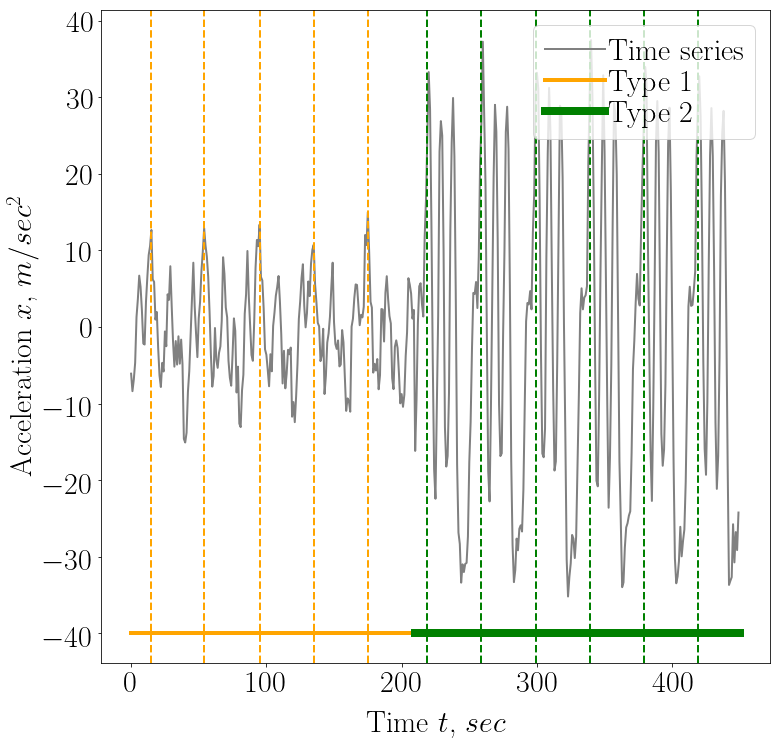
\includegraphics[width=1\textwidth]{results/example}
    \end{column}
    \begin{column}{0.6\textwidth}
        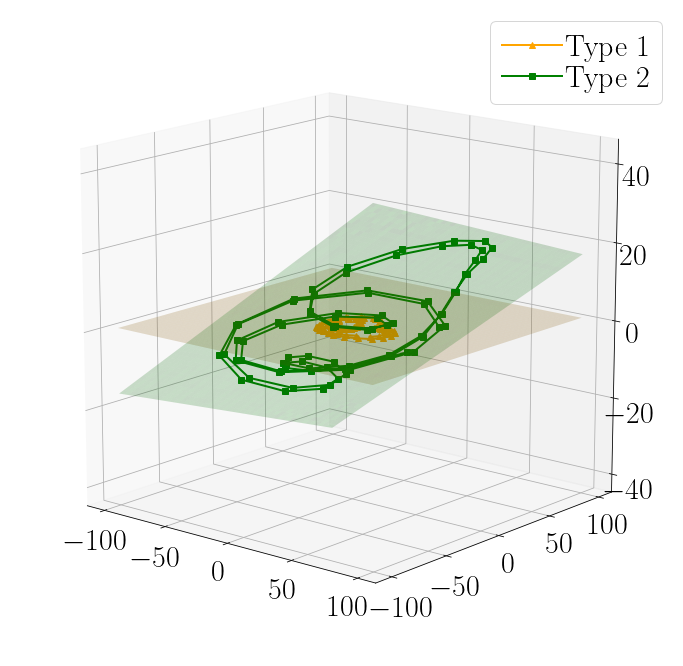
\includegraphics[width=1\textwidth]{results/example_phase}
    \end{column}
\end{columns}

Временной ряд, с разметкой на кластеры: временной ряд с ассесорской разметкой на кластеры и выделением начала квазипериодического сегмента; проекция фазовых траекторий на первые две главные компоненты

\end{frame}

%----------------------------------------------------------------------------------------------------------
\begin{frame}[shrink=5]{Постановка задачи}

\begin{center}
	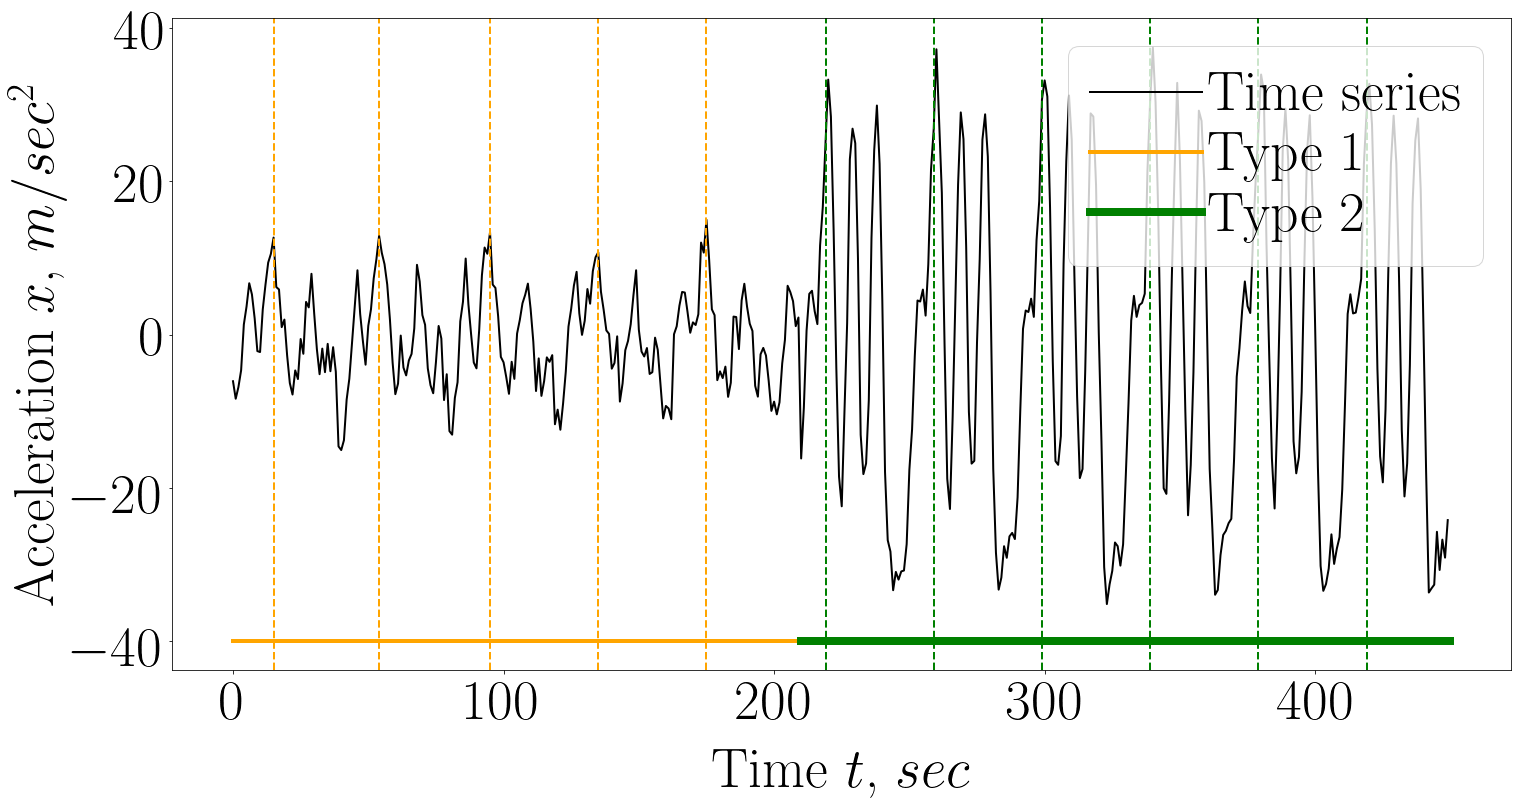
\includegraphics[width=0.6\textwidth]{results/example_slides}
\end{center}

 Задан временной ряд:\\
        $\textbf{x} \in \mathbb{R}^{\text{N}}, \quad \textbf{x} = [\textbf{v}_1, \cdots, \textbf{v}_M], \quad \textbf{v}_i \in \mathcal{V},$\\
        где $\mathcal{V}$ множество возможных сегментов в ряде $\textbf{x}$.

~\\
Предположения:
\begin{itemize}
	\item $\left|\mathcal{V}\right| = K$,
	\item $\textbf{v} \in \mathcal{V}~\left|\textbf{v}\right| \leq T$,
	\item для всех~$i$ либо~$[\textbf{v}_{i-1},\textbf{v}_{i}]$ либо~$[\textbf{v}_{i},\textbf{v}_{i+1}]$  является цепочкой действий,
\end{itemize}
где $\left|\mathcal{V}\right|$ мощность множества сигналов, а $\left|\textbf{v}\right|$ длина сигнала.

\end{frame}

%----------------------------------------------------------------------------------------------------------
\begin{frame}[shrink=5]{Постановка задачи}

Рассматривается отображение
$$
a : t \to \mathbb{Y} = \{1,\cdots, K\}, 
$$
где~$t \in \{1,\cdots, N\}$ некоторый момент времени, на котором задан временной ряд.
Требуется, чтобы отображение~$a$ удовлетворяло следующим свойствам:

$$
\begin{cases}
    a\left(t_1\right) = a\left(t_2\right), &  \text{если в моменты } t_1, t_2 \text{ совершается один тип действий}\\
    a\left(t_1\right) \not= a\left(t_2\right), &  \text{если в моменты } t_1, t_2 \text{ совершаются разные типы действий }
\end{cases}
$$

Пусть задана некоторая асессорская разметка временного ряда:
$$
\textbf{y} \in \{1,\cdots,K\}^{N}.
$$
Тогда ошибка алгоритма~$a$ на временном ряде~$\textbf{x}$ представляется в следующем виде:
$$
S = \frac{1}{N}\sum_{t=1}^{N}[y_t = a\left(t\right)],
$$
где~$t$~---~момент времени,~$y_t$ асессорская разметка~$t$-го момента времени для заданого временного ряда.

\end{frame}
%----------------------------------------------------------------------------------------------------------
\begin{frame}{Кластеризация точек}
Фазовая траектория ряда $\textbf{x}$:
$$\mathbf{H} = \{\textbf{h}_t| \textbf{h}_t = [x_{t-T}, x_{t-T+1}, \cdots, x_{t}],~T\leq t\leq N\},$$
где $\textbf{h}_t$~---~точка фазовой траектории.

~\\
Фазовые подпространства:
$$\mathbf{S} = \{\textbf{s}_t| \textbf{s}_t = [\textbf{h}_{t-T}, \textbf{h}_{t-T+1}, \cdots, \textbf{h}_{t+T-1}],~T\leq t\leq N-T\},$$
где $\textbf{s}_t$~---~это сегмент фазовой траектории.

~\\
Множество базисов:
$$\mathbf{W} = \{\textbf{W}_t| \textbf{W}_t = [\lambda^1_t\textbf{w}^1_t, \lambda^2_t\textbf{w}^2_t]\}, \quad \bm{\Lambda} = \{\bm{\lambda}_t| \bm{\lambda}_t=[\lambda^1_t, \lambda^2_t]\},$$
где~$[\textbf{w}^1_t, \textbf{w}^2_t]$ и~$[\lambda^1_t, \lambda^2_t]$ это базисные векторы и соответствующие им собственные числа для сегмента фазовой траектории~$\textbf{s}_t$.
\end{frame}
%----------------------------------------------------------------------------------------------------------
\begin{frame}[shrink=5]{Кластеризация точек}
Расстояние между элементами~$\mathbf{W}_{t_1},\mathbf{W}_{t_2}$:\\
$$\rho\left(\textbf{W}_1, \textbf{W}_2\right) = \max\left(\max_{\textbf{e}_2 \in \textbf{W}_2} d_{1}\left(\textbf{e}_2\right), \max_{\textbf{e}_1 \in \textbf{W}_1} d_{2}\left(\textbf{e}_1\right)\right),$$
где ~$\textbf{e}_i$ это базисный вектор пространства~$\textbf{W}_i,$ а~$d_i\left(\textbf{e}\right)$ является расстоянием от вектора~$\textbf{e}$ до пространства~$\textbf{W}_i$.

\begin{theorem}
Пусть задано множество подпространств~$\mathbb{W}$ пространства~$\mathbb{R}^{n}$. Каждое подпространство которого задается базисом~$\mathbf{W}_i\in \mathbf{W}$, тогда функция расстояния~$\rho\left(\textbf{W}_1, \textbf{W}_2\right)$ является метрикой заданой на множестве базисов~$\mathbf{W}$:
$$
\rho\left(\textbf{W}_1, \textbf{W}_2\right) = \max\left(\max_{\textbf{e}_2 \in \textbf{W}_2} d_{1}\left(\textbf{e}_2\right), \max_{\textbf{e}_1 \in \textbf{W}_1} d_{2}\left(\textbf{e}_1\right)\right),
$$
где~$\textbf{e}_i$ это базисный вектор из~$\textbf{W}_i$, a~$d_i\left(\textbf{e}\right)$ является расстоянием от вектора~$\textbf{e}$ до пространства заданого базисом~$\textbf{W}_i$.
\end{theorem}
\end{frame}

%----------------------------------------------------------------------------------------------------------

\begin{frame}[shrink=5]{Кластеризация точек}
Расстояние между элементами~$\mathbf{W}_{t_1},\mathbf{W}_{t_2}$:\\
$$
\rho\left(\textbf{W}_1, \textbf{W}_2\right) = \max_{\{\textbf{a},\textbf{b},\textbf{c}\} \subset \textbf{W}_1\cup \textbf{W}_2 } V\left(\textbf{a},\textbf{b},\textbf{c}\right), 
$$
где~$\textbf{W}_1\cup\textbf{W}_2$ это объединение базисных векторов первого и второго пространства,~$V\left(\textbf{a},\textbf{b},\textbf{c}\right)$~---~объем параллелепипеда построенного на векторах~$\textbf{a}, \textbf{b}, \textbf{c}$, которые являются столбцами матрицы~$\textbf{W}_1\cup\textbf{W}_2$.

~\\
Расстояние между элементами $\mathcal{L}$:\\
$$
\rho\left(\bm{\lambda}_1, \bm{\lambda}_2\right) = \sqrt[]{\left(\bm{\lambda}_1 - \bm{\lambda}_2\right)^{\mathsf{T}}\left(\bm{\lambda}_1 - \bm{\lambda}_2\right)}.
$$

~\\
Расстояние между точками временного ряда:\\
$$
\rho\left(t_1, t_2\right) = \rho\left(\textbf{W}_1, \textbf{W}_2\right) + \rho\left(\bm{\lambda}_1, \bm{\lambda}_2\right).
$$

~\\
Матрица попарных растояний:\\
$$\textbf{M} = \mathbb{R}_{+}^{N\times N}.$$

\end{frame}
%----------------------------------------------------------------------------------------------------------


\begin{frame}{Описание временных рядов в эксперименте}

\begin{tabular}{|c|c|c|c|}
\hline
	Ряд,~$\textbf{x}$&Точек,~$N$&Сегментов,~$K$&Период,~$T$\\
	\hline
	\multicolumn{1}{|l|}{Physical~Motion~1}
	& 900& 2& 40\\
	\hline
	\multicolumn{1}{|l|}{Physical~Motion~2}
	& 900& 2& 40\\
	\hline
	\multicolumn{1}{|l|}{Synthetic~1}
	& 2000& 2& 20\\
	\hline
	\multicolumn{1}{|l|}{Synthetic~2}
	& 2000& 3& 20\\
	\hline
	\multicolumn{1}{|l|}{Simple~1}
	& 1000& 2& 100\\
\hline

\end{tabular}

\begin{itemize}
	\item $N$ --- число точек во временном ряде,
	\item $K$ --- число различных действий во временном ряде,
	\item $T$ --- максимальная длина сегмента.
\end{itemize}

\end{frame}
%----------------------------------------------------------------------------------------------------------
\begin{frame}[shrink=5]{Пример временных рядов}

\begin{columns}
    \begin{column}{0.5\textwidth}
        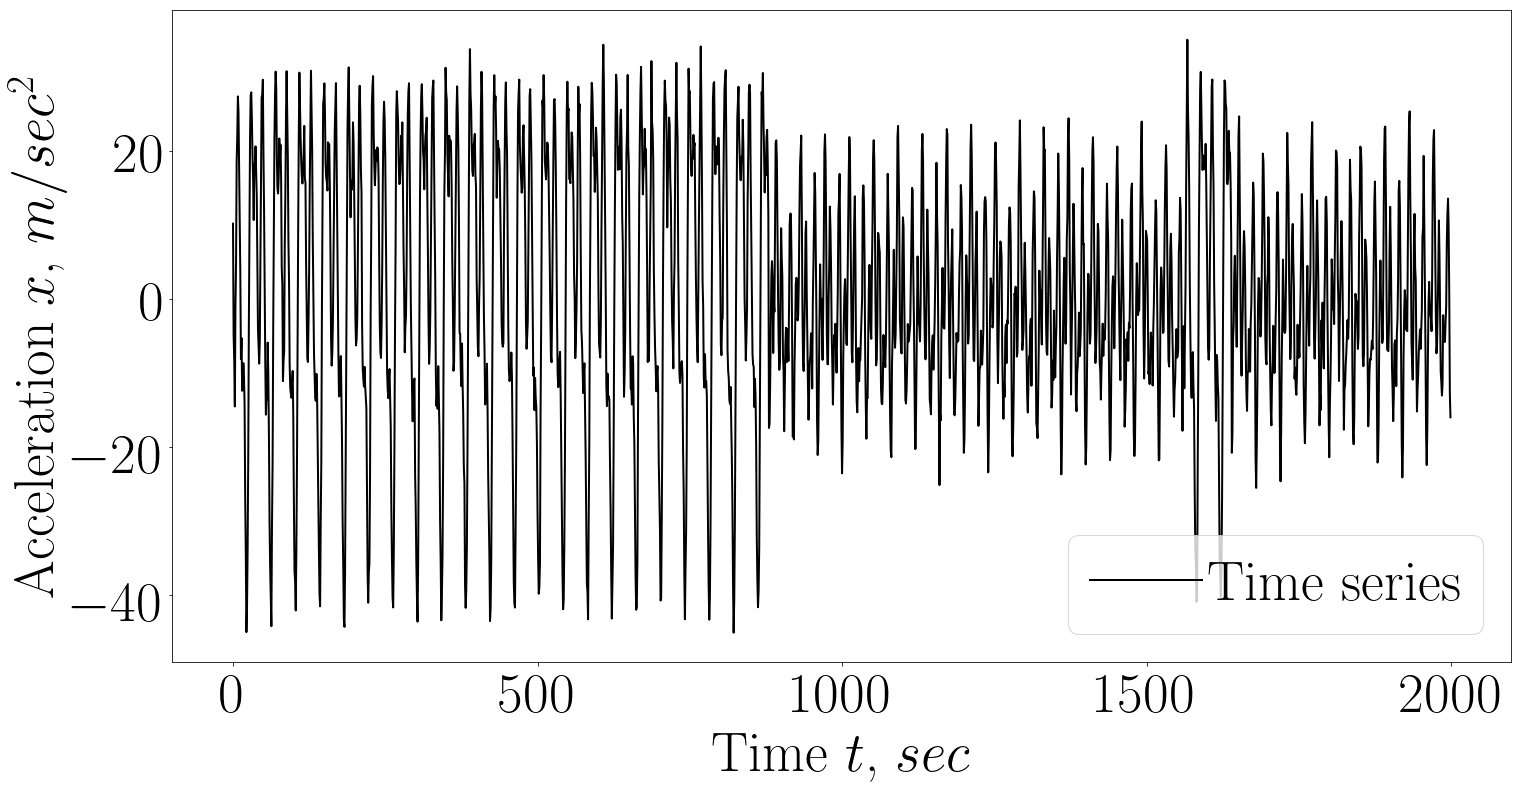
\includegraphics[width=1\textwidth]{results/2_patern_2_series}
    \end{column}
    \begin{column}{0.5\textwidth}
        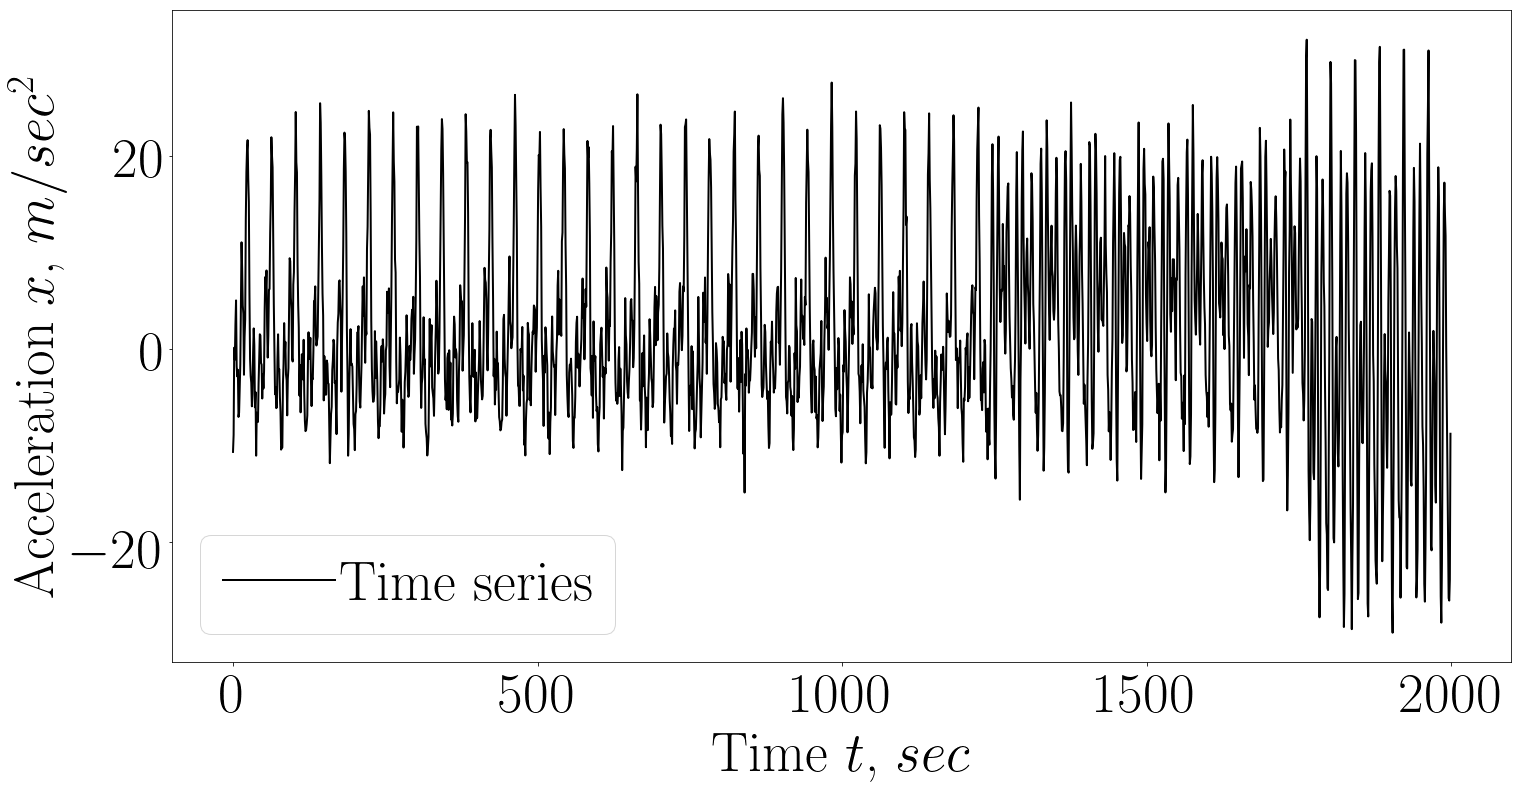
\includegraphics[width=1\textwidth]{results/3_patern_2_series}
    \end{column}
\end{columns}

\begin{columns}
    \begin{column}{0.5\textwidth}
        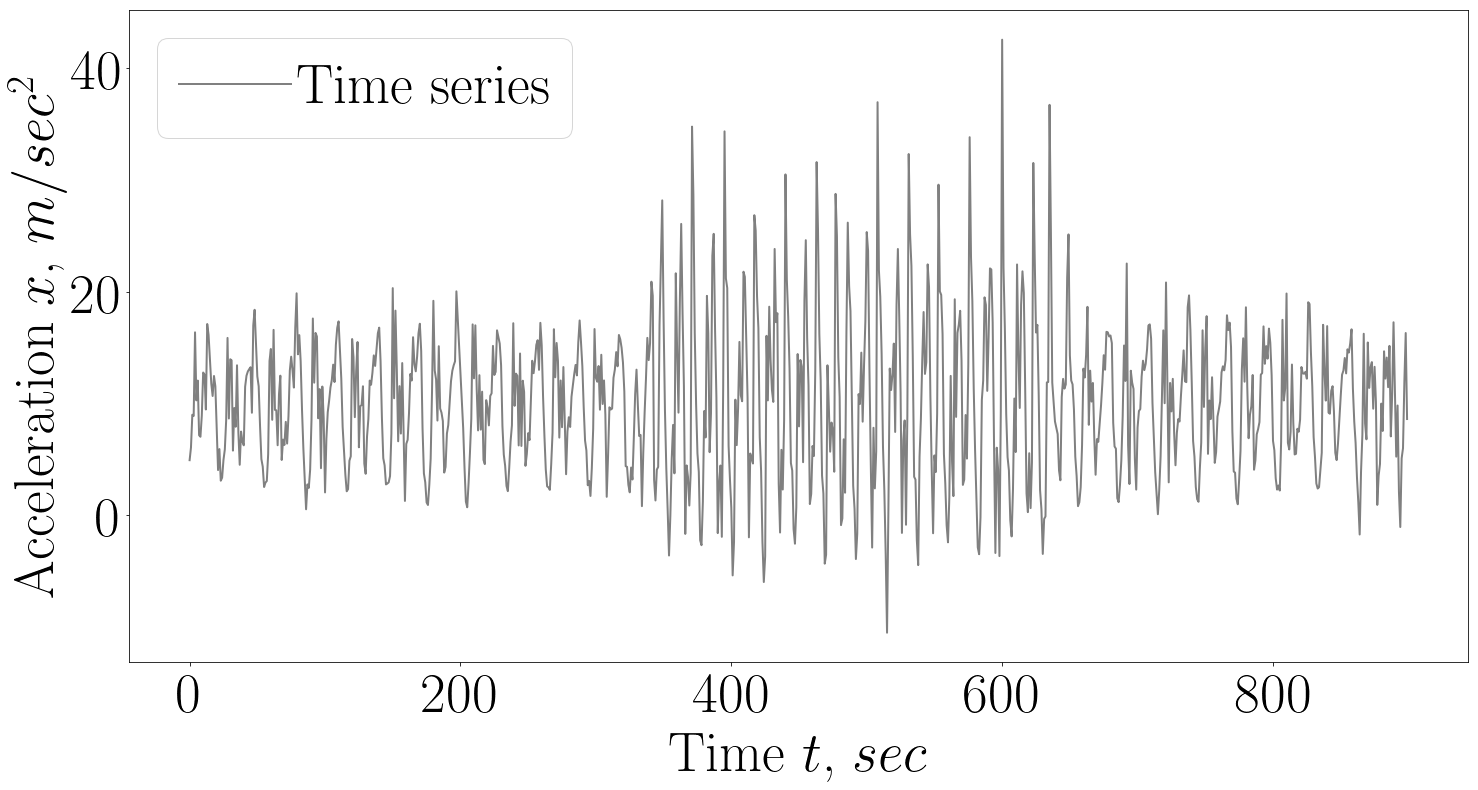
\includegraphics[width=1\textwidth]{results/real_1_series}
    \end{column}
    \begin{column}{0.5\textwidth}
        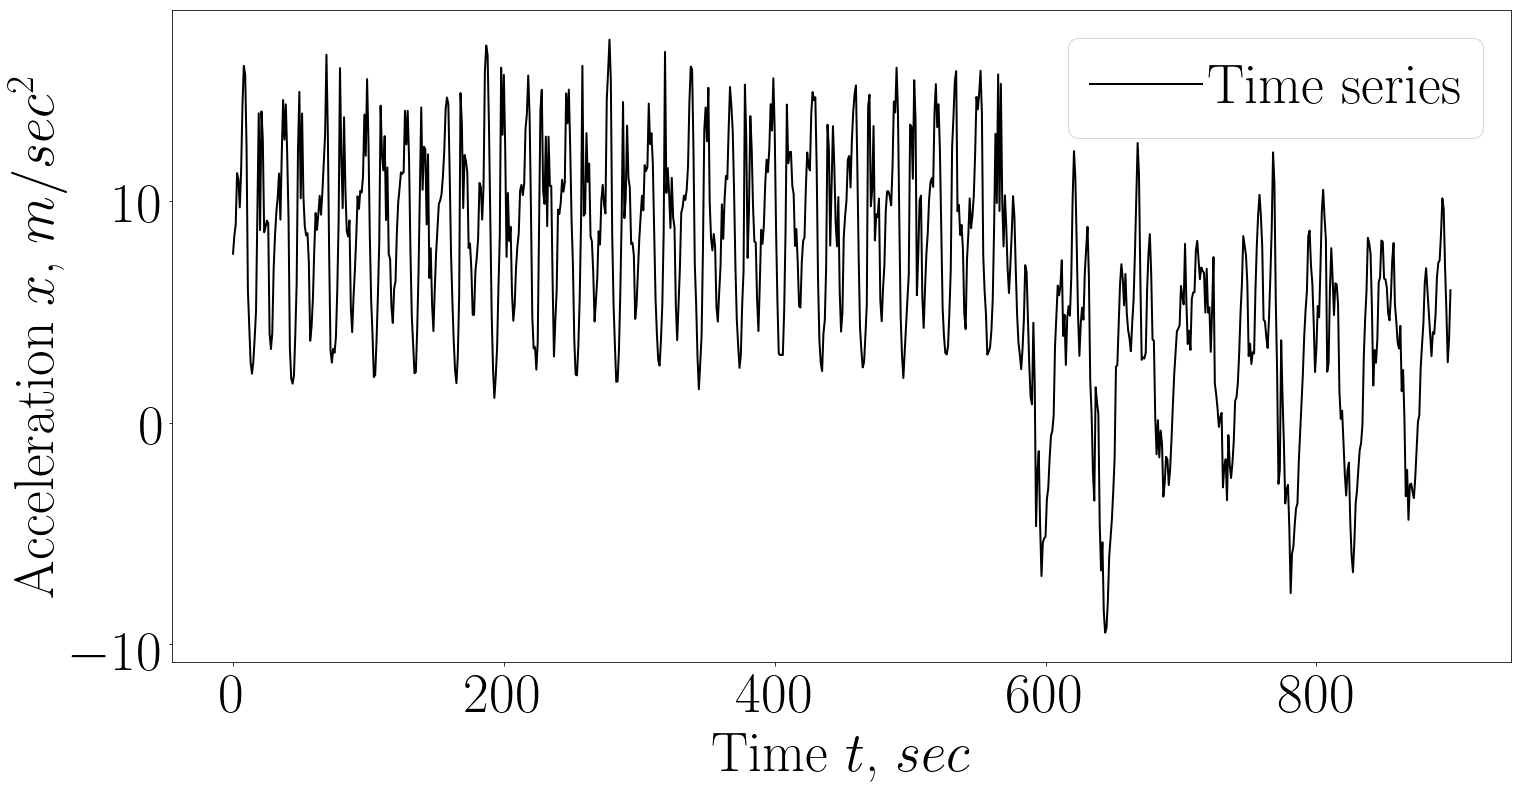
\includegraphics[width=1\textwidth]{results/real_2_series}
    \end{column}
\end{columns}

Временные ряды построенные синтетически, а также при помощи мобильного акселерометра.

\end{frame}
%----------------------------------------------------------------------------------------------------------
\begin{frame}[shrink=5]{Матрица попарных расстояний $\textbf{M}$}

\begin{columns}
    \begin{column}{0.35\textwidth}
        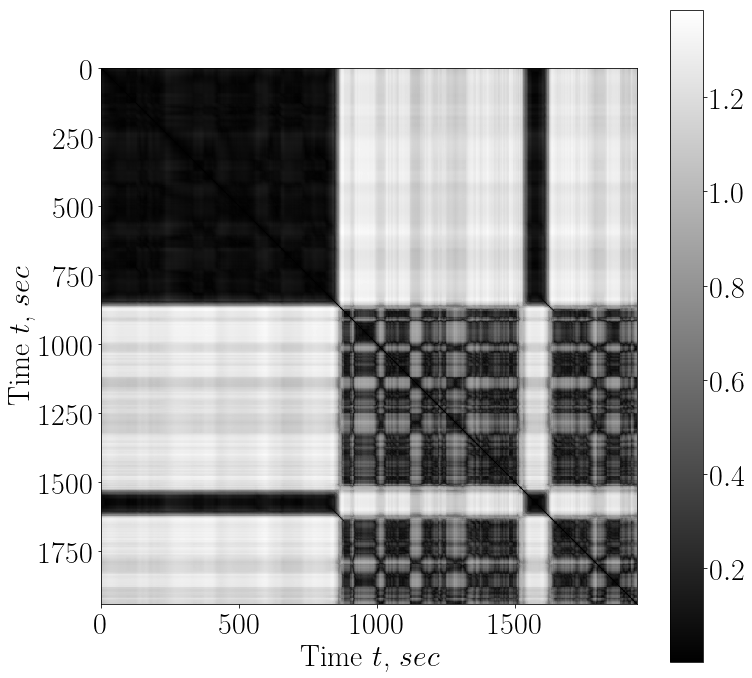
\includegraphics[width=1\textwidth]{results/2_patern_2_full}
    \end{column}
    \begin{column}{0.35\textwidth}
        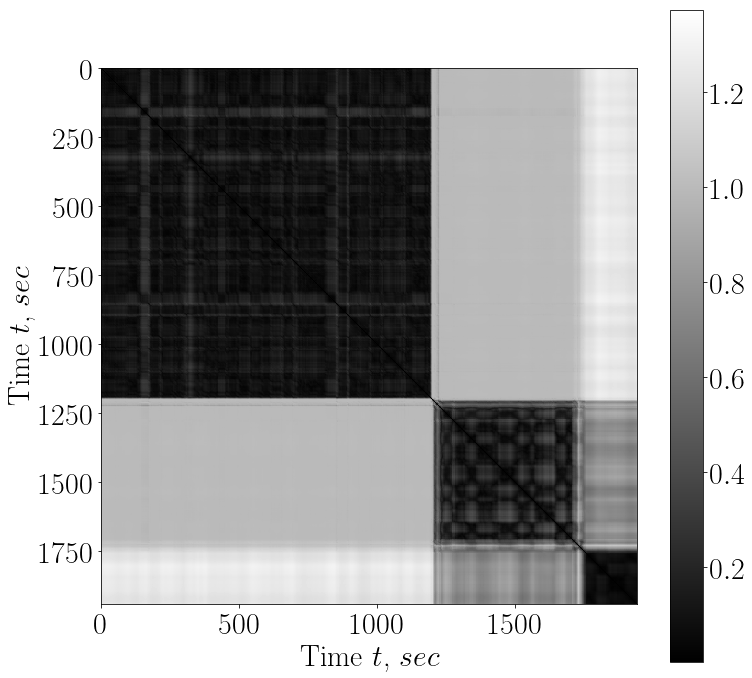
\includegraphics[width=1\textwidth]{results/3_patern_2_full}
    \end{column}
\end{columns}

\begin{columns}
    \begin{column}{0.35\textwidth}
        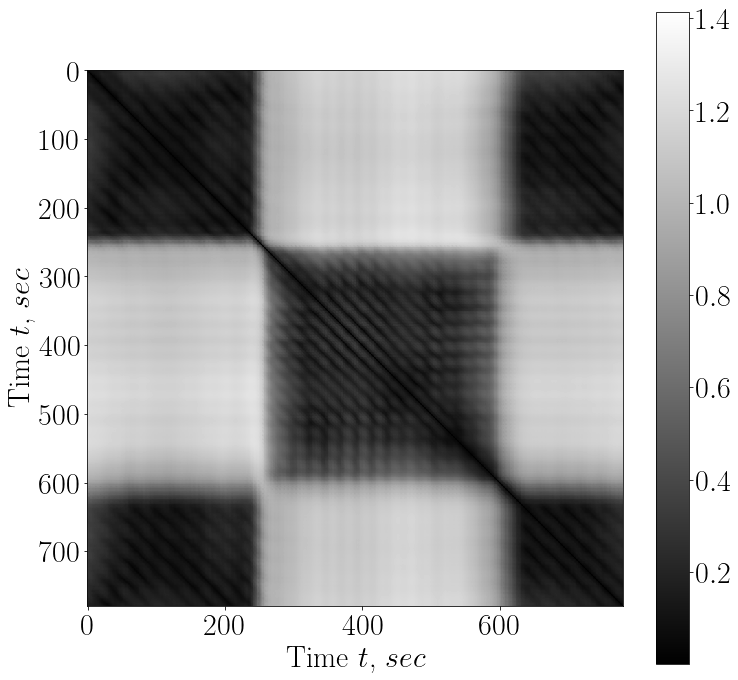
\includegraphics[width=1\textwidth]{results/real_1_full}
    \end{column}
    \begin{column}{0.35\textwidth}
        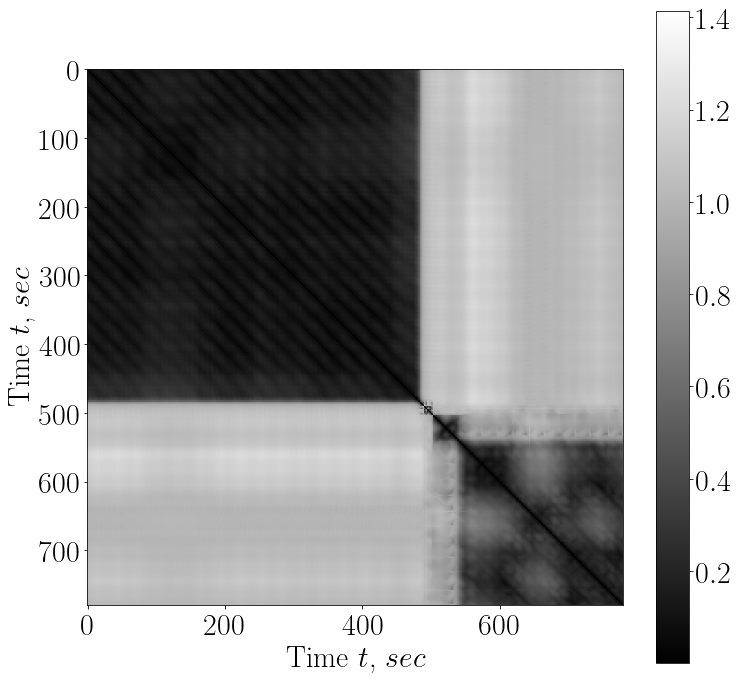
\includegraphics[width=1\textwidth]{results/real_2_full}
    \end{column}
\end{columns}

Матрицы попарных расстояний для временных рядов, построенных синтетически, а также при помощи мобильного акселерометра.

\end{frame}
%----------------------------------------------------------------------------------------------------------
\begin{frame}[shrink=5]{Проекция точек фазовой траектории на плоскость}

\begin{columns}
    \begin{column}{0.35\textwidth}
        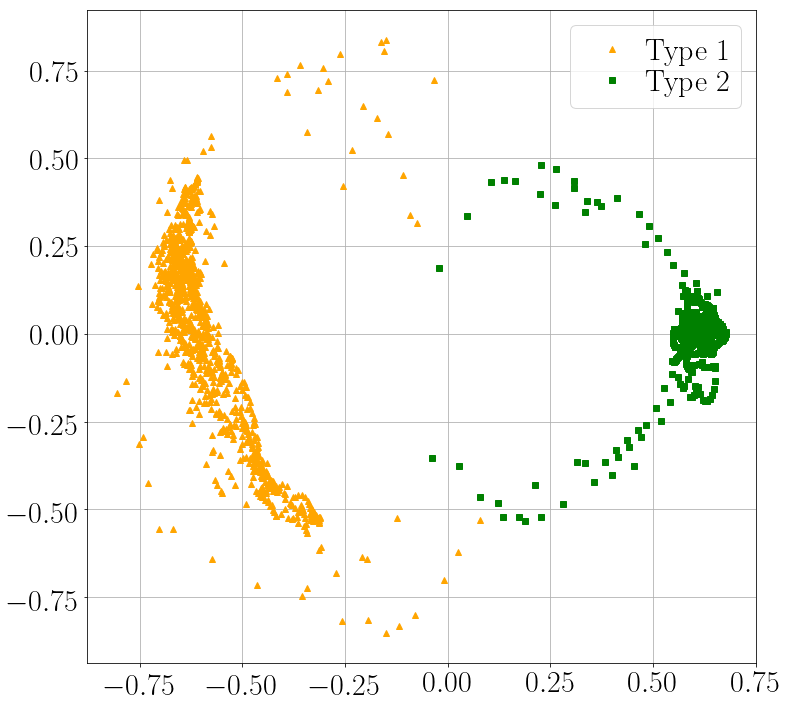
\includegraphics[width=1\textwidth]{results/2_patern_2_2D_vector}
    \end{column}
    \begin{column}{0.35\textwidth}
        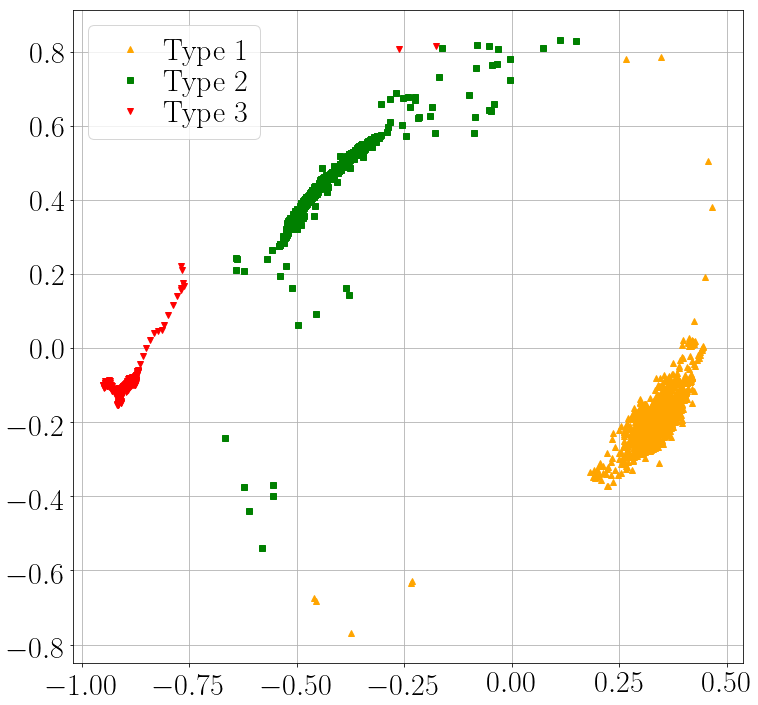
\includegraphics[width=1\textwidth]{results/3_patern_2_2D_vector}
    \end{column}
\end{columns}

\begin{columns}
    \begin{column}{0.35\textwidth}
        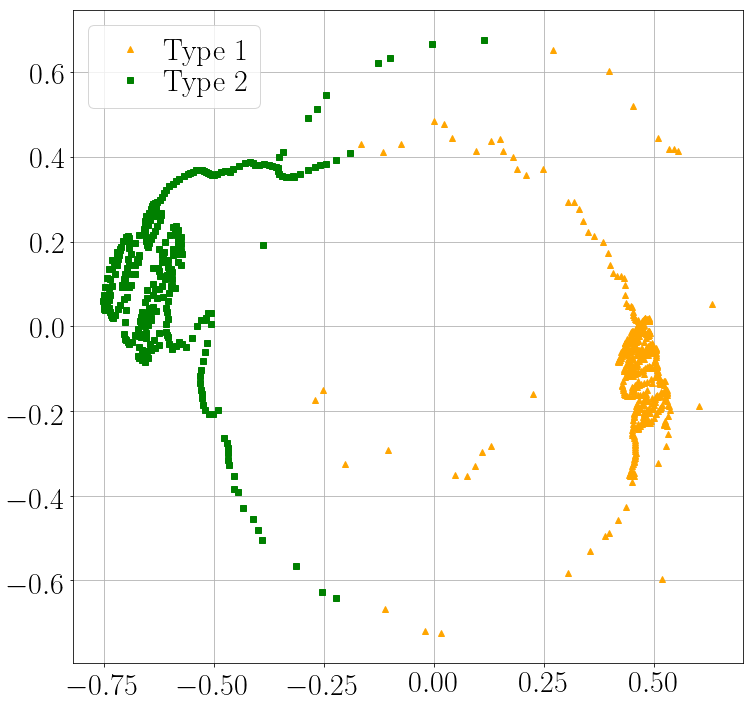
\includegraphics[width=1\textwidth]{results/real_1_2D_vector}
    \end{column}
    \begin{column}{0.35\textwidth}
        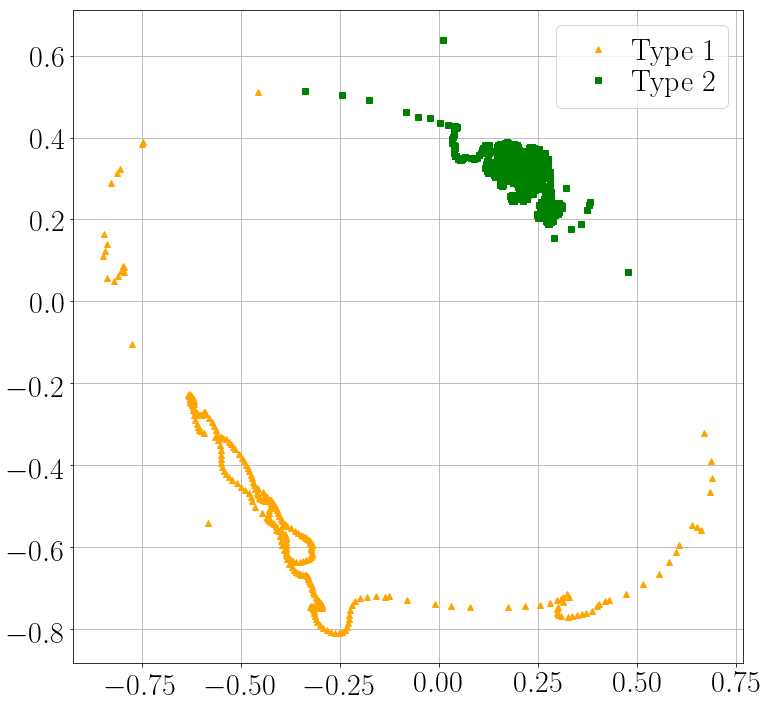
\includegraphics[width=1\textwidth]{results/real_2_2D_vector}
    \end{column}
\end{columns}

Иллюстрация проекции признакового описания точек временного ряда на плоскости для временных рядов, построенных синтетически, а также при помощи мобильного акселерометра.

\end{frame}
%----------------------------------------------------------------------------------------------------------
\begin{frame}[shrink=5]{Кластеризация точек временного ряда}

\begin{columns}
    \begin{column}{0.5\textwidth}
        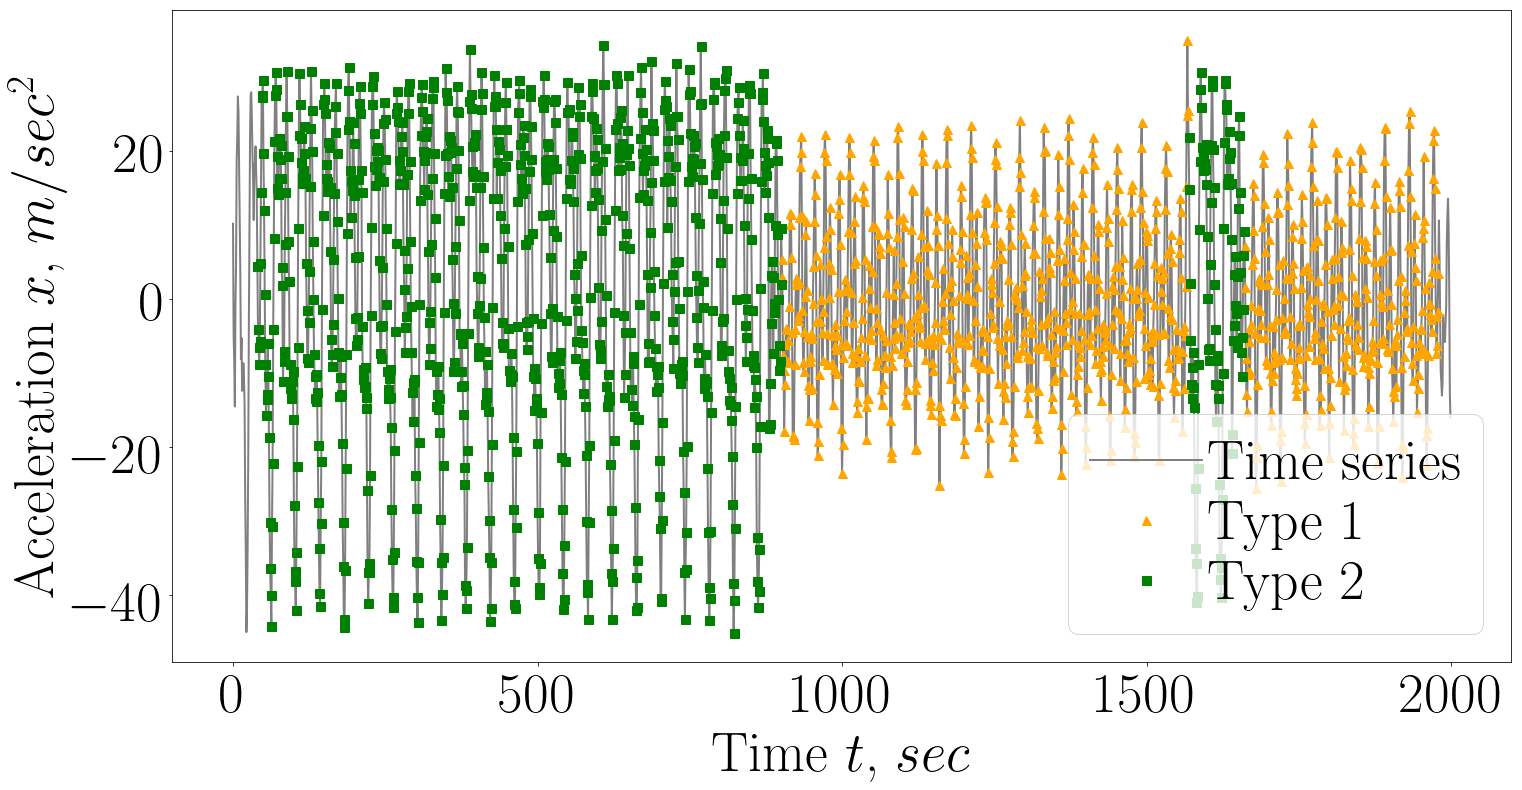
\includegraphics[width=1\textwidth]{results/2_patern_2_claster_vector}
    \end{column}
    \begin{column}{0.5\textwidth}
        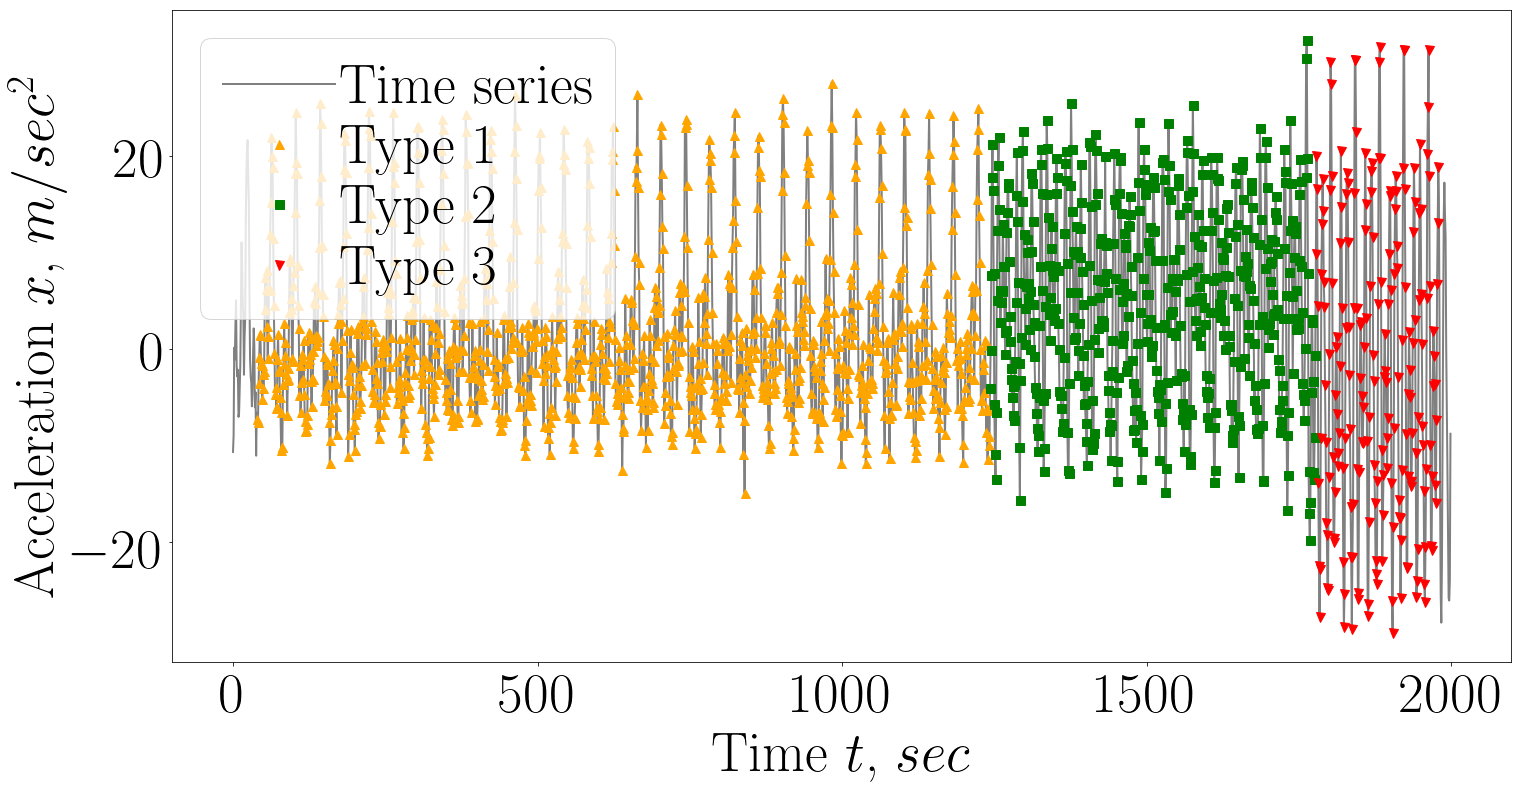
\includegraphics[width=1\textwidth]{results/3_patern_2_claster_vector}
    \end{column}
\end{columns}

\begin{columns}
    \begin{column}{0.5\textwidth}
        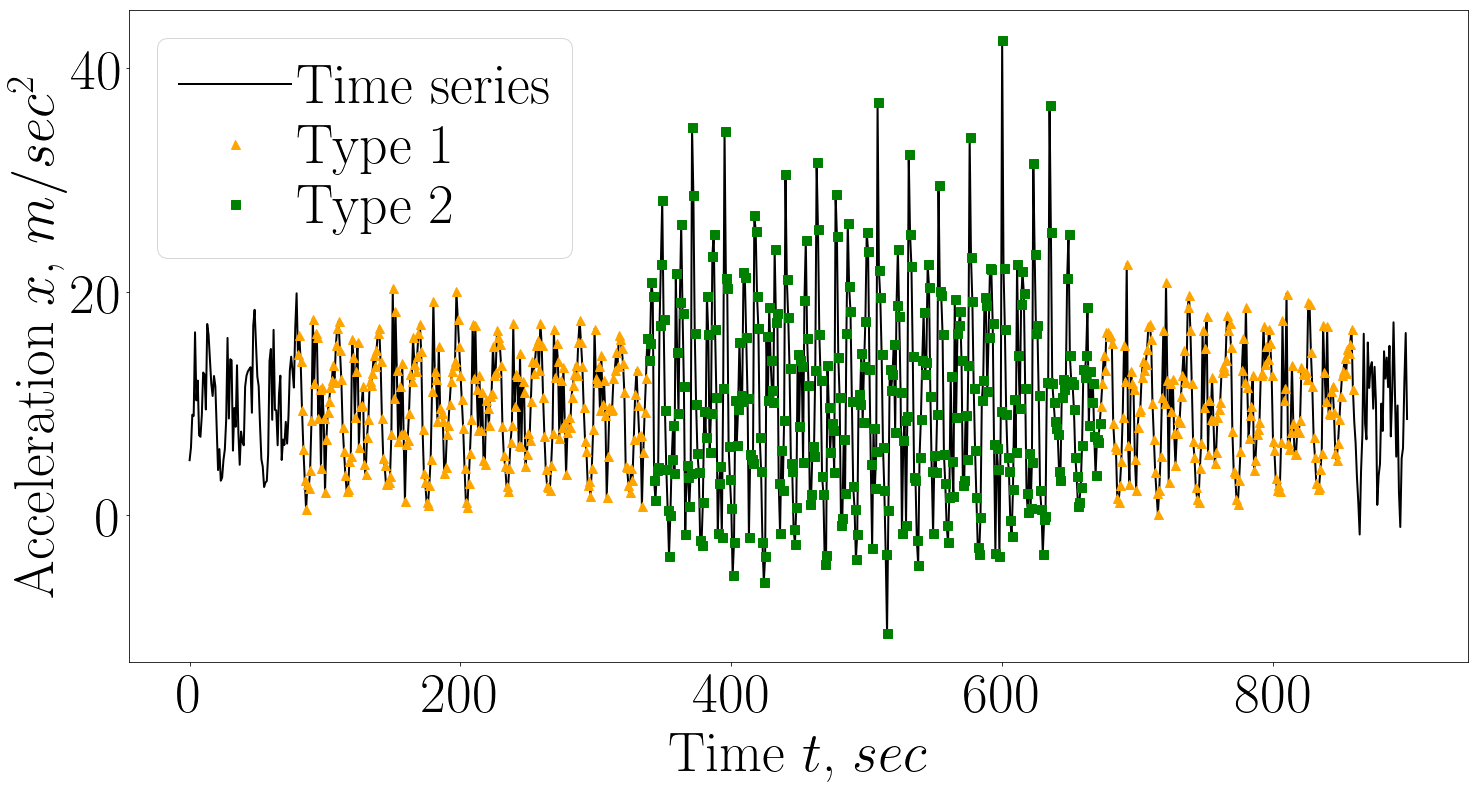
\includegraphics[width=1\textwidth]{results/real_1_claster_vector}
    \end{column}
    \begin{column}{0.5\textwidth}
        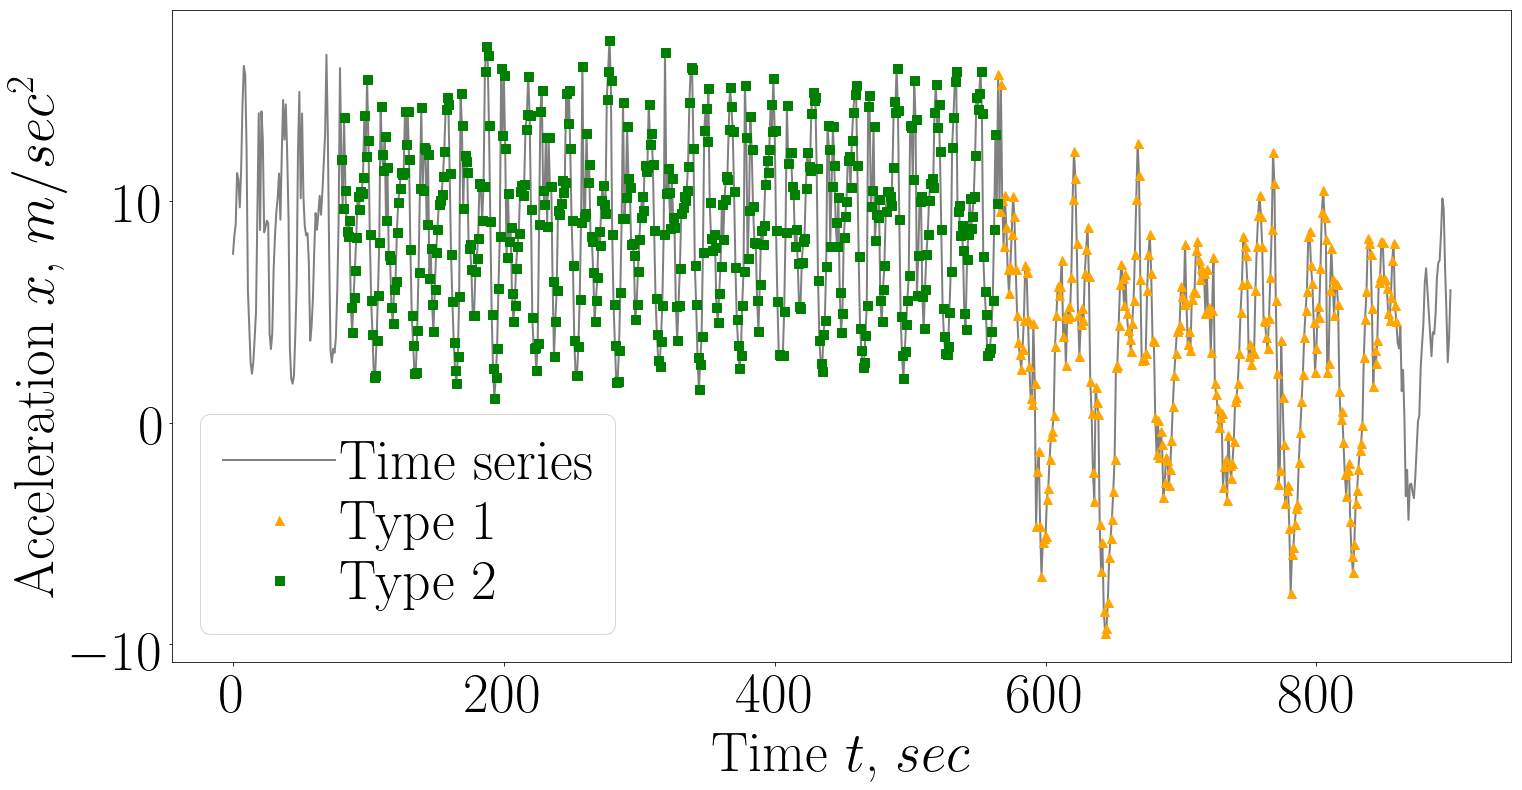
\includegraphics[width=1\textwidth]{results/real_2_claster_vector}
    \end{column}
\end{columns}

Результат кластеризации точек временных рядов, построенных синтетически, а также при помощи мобильного акселерометра.

\end{frame}
%----------------------------------------------------------------------------------------------------------
\begin{frame}{Результаты работы алгоритма кластеризации}

\begin{tabular}{|c|c|c|c|c|}
\hline
	Ряд,~$\textbf{x}$ &Длина,~$N$& Сегментов,~$K$&Длина,~$T$& Ошибка,~$S$\\
	\hline
	\multicolumn{1}{|l|}{Phys.~Motion~1}
	& 900& 2& 40& 0.06\\
	\hline
	\multicolumn{1}{|l|}{Phys.~Motion~2}
	& 900& 2& 40& 0.03\\
	\hline
	\multicolumn{1}{|l|}{Synthetic~1}
	& 2000& 2& 20& 0.04\\
	\hline
	\multicolumn{1}{|l|}{Synthetic~2}
	& 2000& 3& 20& 0.03\\
\hline
\end{tabular}

\begin{itemize}
	\item $N$ --- число точек во временном ряде,
	\item $K$ --- число различных действий во временном ряде,
	\item $T$ --- максимальная длина сегмента,
	\item $S$ --- точность кластеризации.
\end{itemize}

\end{frame}
%----------------------------------------------------------------------------------------------------------
\begin{frame}[shrink=5]{Сегментация временных рядов}

\begin{columns}
    \begin{column}{0.5\textwidth}
        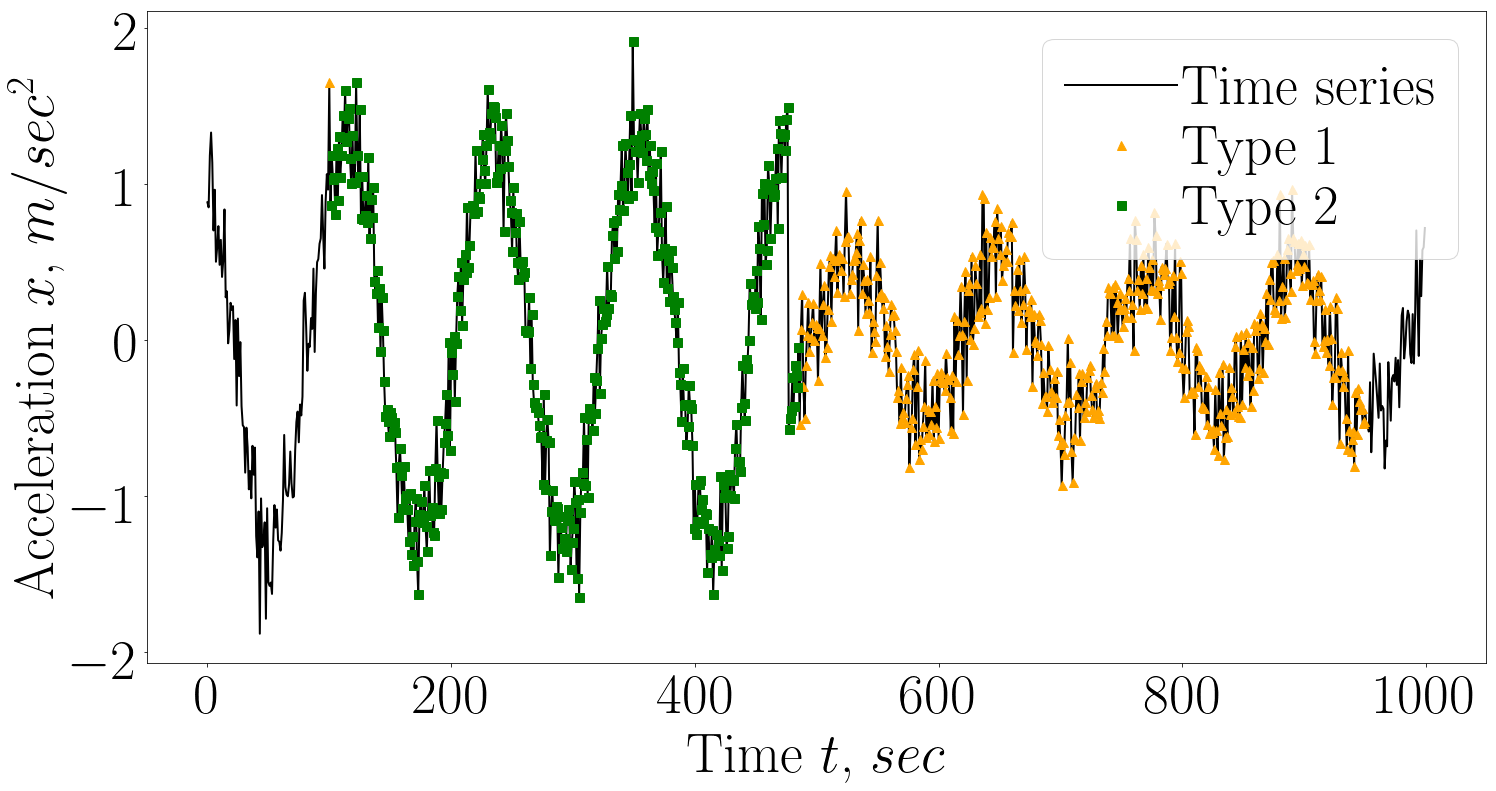
\includegraphics[width=1\textwidth]{results/simple_1_claster_vector}
    \end{column}
    \begin{column}{0.3\textwidth}
        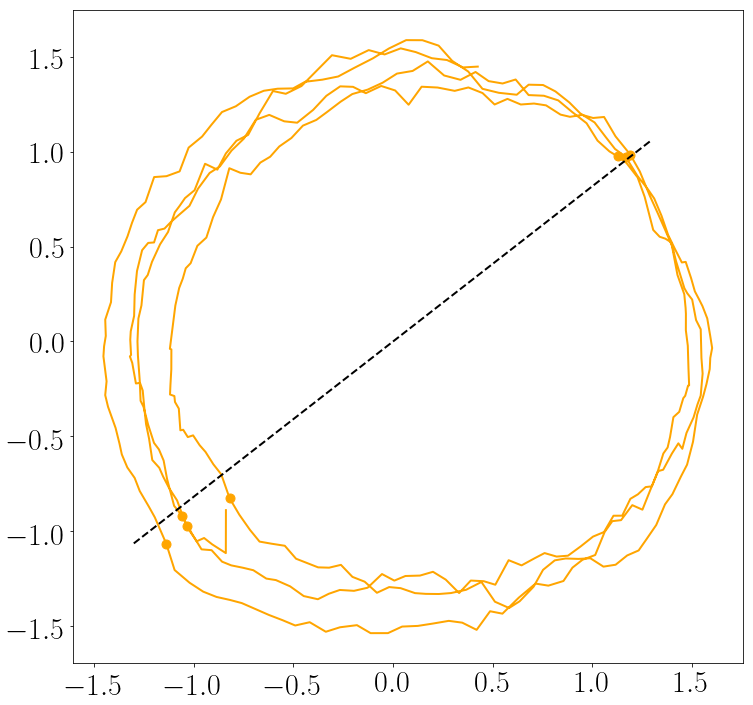
\includegraphics[width=1\textwidth]{results/simple_1_phase_space0}
    \end{column}
\end{columns}

\begin{columns}
    \begin{column}{0.5\textwidth}
        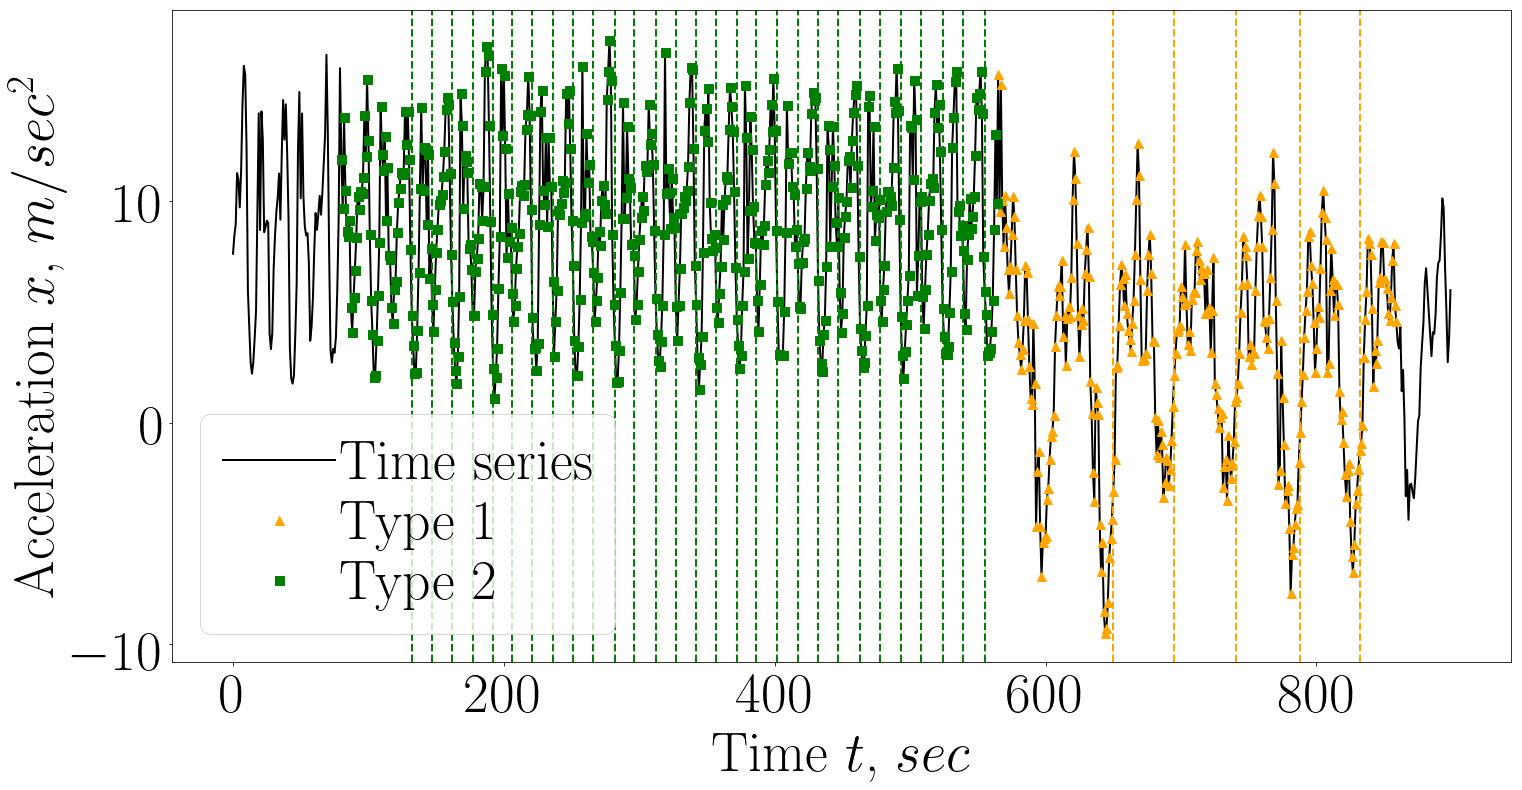
\includegraphics[width=1\textwidth]{results/real_2_segmentation_vector}
    \end{column}
    \begin{column}{0.3\textwidth}
        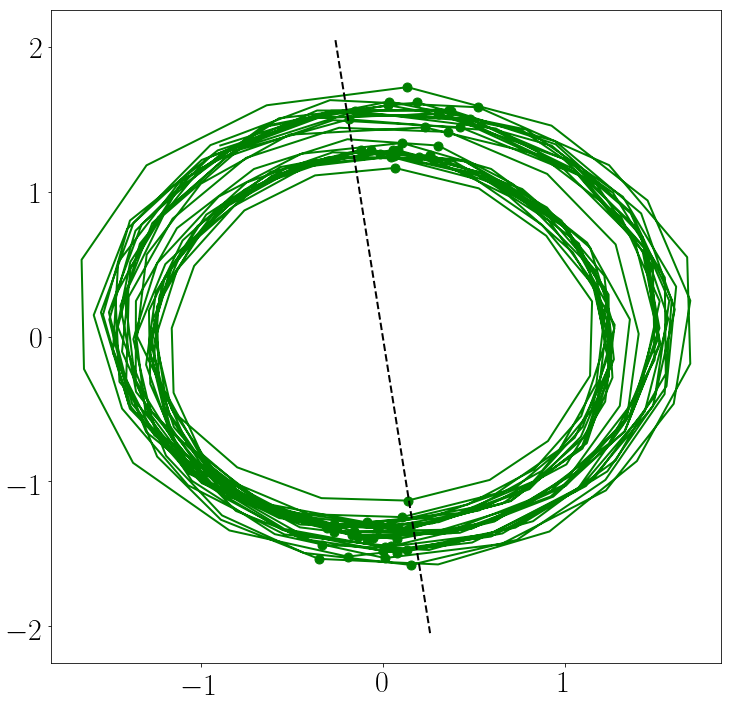
\includegraphics[width=1\textwidth]{results/real_2_phase_space1}
    \end{column}
\end{columns}

Результат сегментации временных рядов, в случае двух синусоидальных сигналов в произвольной частотой и амплитудой, а также в случае реальных данных, полученных при помощи акселерометра.

\end{frame}
%----------------------------------------------------------------------------------------------------------

\begin{frame}[shrink=5]{Заключение}
	\begin{itemize}
		\item Предложен алгоритм поиска характерных сегментов, который основывается на методе главных компонент для локального снижения размерности
		\item Введена функция расстояния между локальными базисами в каждый момент времени, которые интерпретировались как признаковое описание точки временного ряда. Данная функция является метрикой.
		\item В ходе эксперимента, на реальных показаниях акселерометра, а также на синтетических данных, было показано, что предложенный метод измерение расстояния между базисами хорошо разделяет точки которые принадлежат различным действиям, что приводит к хорошей кластеризации объектов.
		\item Также в эксперименте была проведена полная сегментация временных рядов для каждого кластера по отдельности.
	\end{itemize}
	
	\begin{itemize}
		\item Планируется решить задачу нахождения минимального размера фазового пространства, для которого  фазовая траектория не имеет самопересечений.
	\end{itemize}
\end{frame}
%----------------------------------------------------------------------------------------------------------
\begin{frame}{Публикации}
	\begin{itemize}
		\item \textit{Грабовой А. В., Стрижов В. В.} Анализ свойств локальных моделей в задачах кластеризации квазипериодических временных рядов // (в процессе)
		\item \textit{Грабовой А. В., Бахтеев О. Ю., Стрижов В. В.} Определение релевантности параметров нейросети // Информатика и ее применения, 2019, 13(2).
		\item \textit{Гадаев Т. Т., Грабовой А. В., Мотренко А. П., Стрижов В. В.} Численные методы оценки объема выборки в задачах регрессии и классификации //(в процессе)
		\item \textit{Бучнев Т. Т., Грабовой А. В., Гадаев Т. Т., Стрижов В. В.} Ранее прогнозирование достаточного объема выборки для обобщенно линейной модели // (в процессе)
	\end{itemize}
\end{frame}
%----------------------------------------------------------------------------------------------------------

\end{document} 